%!TEX TS-program = ../make.zsh

\begin{frame}[fragile]{Example scan for best hole-ice parameters based on calibration data}
  \begin{column}{0.5\textwidth}
    \raisebox{-1.5cm}{%
      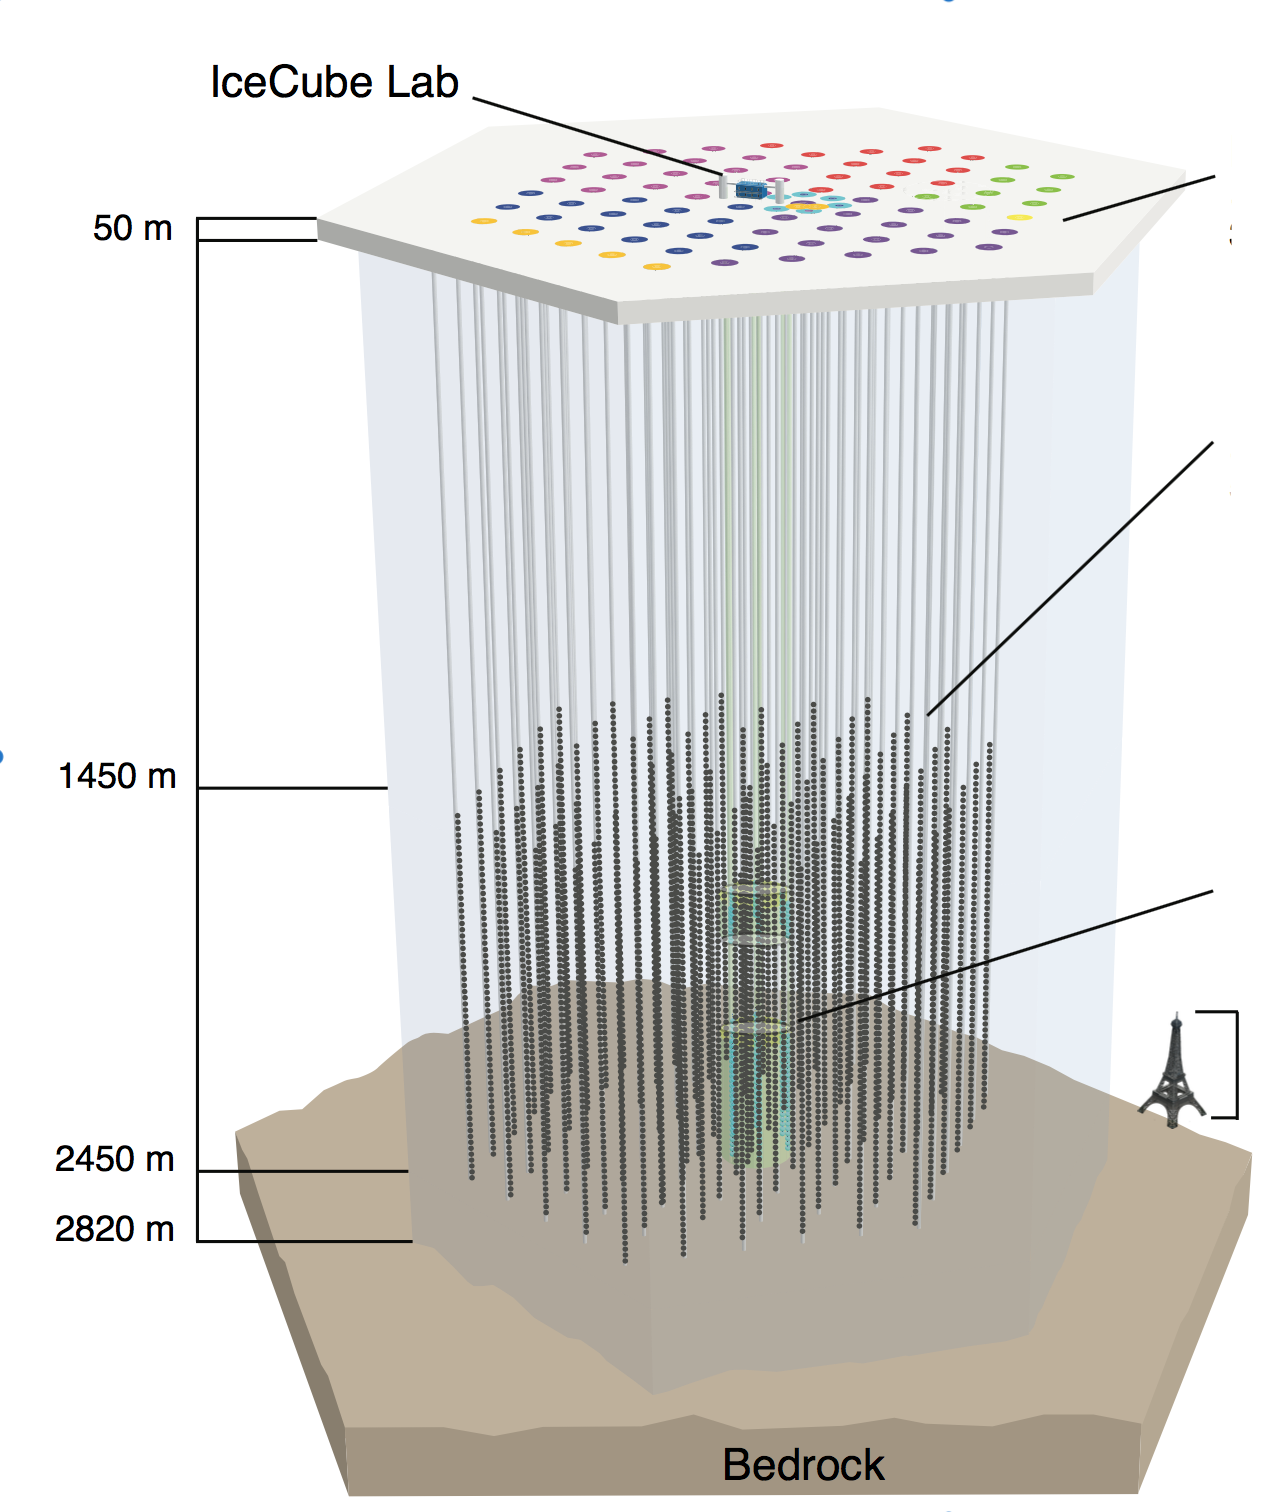
\includegraphics[width=0.3\textwidth]{img/icecube-schematics-instrumentation-min}}
    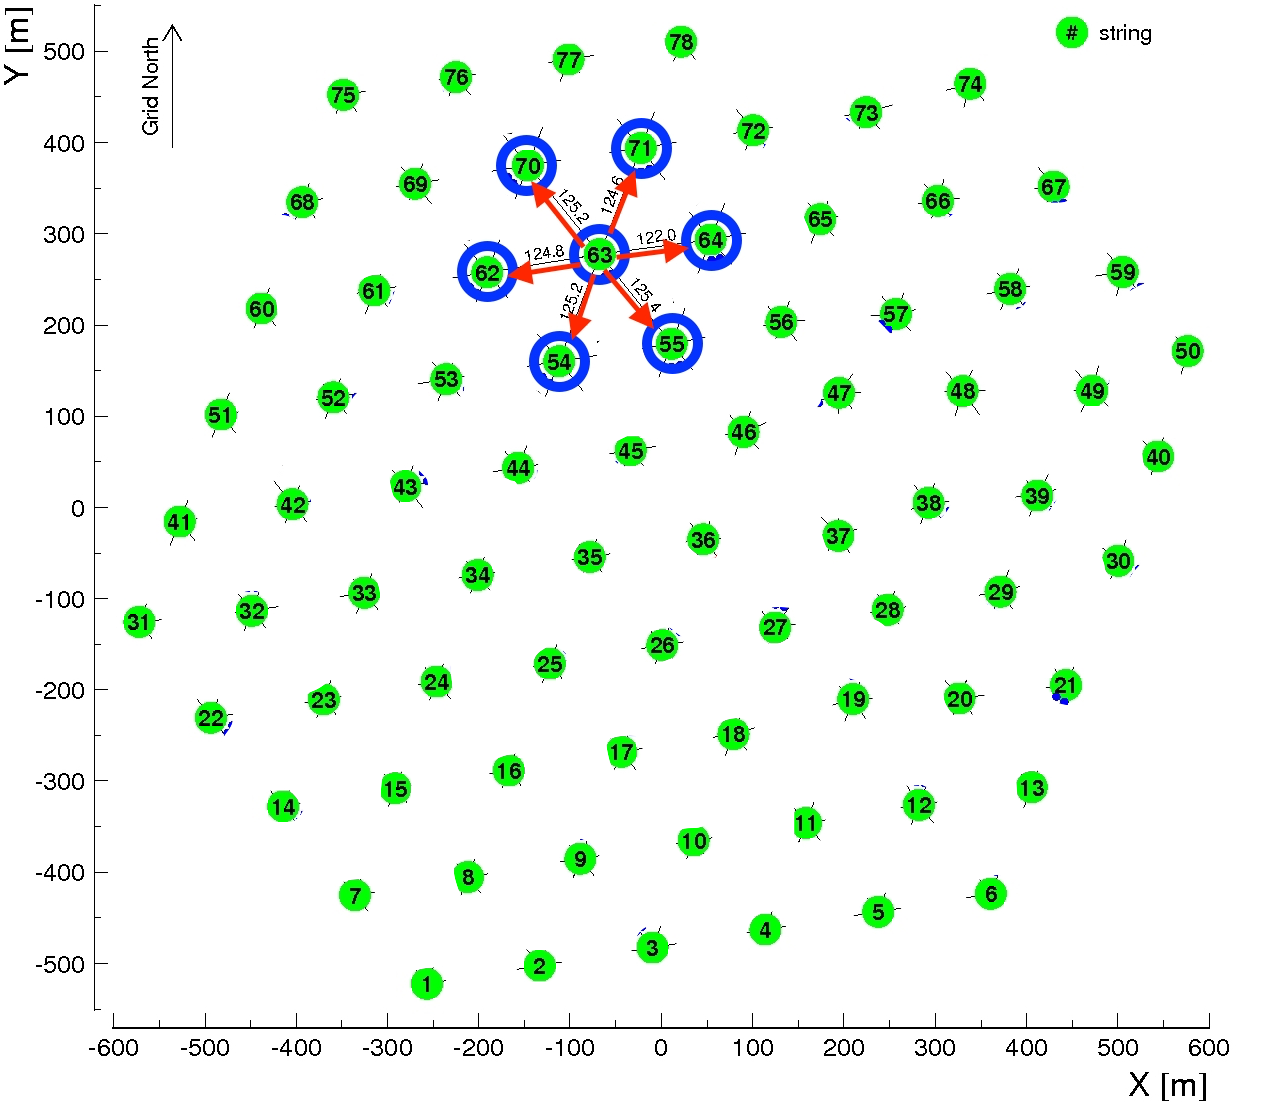
\includegraphics[width=0.9\textwidth]{img/flasher-scenario-light}

  \end{column}
  \begin{column}{0.5\textwidth}
    \image{flasher-contours-59}
  \end{column}

  \source{\url{https://github.com/fiedl/hole-ice-study/issues/59}. Footprint based on \url{https://wiki.icecube.wisc.edu/index.php/File:Distances.i86.jpg}. Image: Aartsen et al., The IceCube Neutrino Observatory: Instrumentation and online systems, 2017.}
\end{frame}

% \begin{frame}[fragile]{Flasher parameter scan vs. SpiceHD scan}
%   \begin{column}{0.5\textwidth}
%     SpiceHD with ppc: \medskip
%
%     \image{flasher-contours-martin}
%
%     DOM positions are fit parameters.
%   \end{column}
%   \begin{column}{0.5\textwidth}
%     clsim with direct hole ice: \medskip
%
%     \image{flasher-same-color-axis-as-spicehd}
%
%     All DOMs perfectly centered within hole ice.
%   \end{column}
%
%   \bigskip
%   Mind systematics: DOM displacement does account for the observed scattering-length factor $\frac{1}{3}$ for the hole-ice radius of 1.8 dom radii (right-hand side of the plot).
%
%   \source{\url{https://github.com/fiedl/hole-ice-study/issues/106}. }
% \end{frame}